\section{DNN Acceleration Fault Analysis Platform and Fault Classification}
\label{sec:fault-analysis}
\subsection{Fault Analysis Platform}
To conduct systematic analysis of faults on a DNN acceleration 
system, we build a fault analysis platform on Xilinx Zynq (ARM-FPGA) 
as shown in Figure \ref{fig:fault-analysis-overview}. It has a 
typical neural network accelerator implemented on FPGA. The accelerator 
is attached to the ARM processor in Zynq with AXI bus. Typically, the ARM processor 
can set up the neural network parameters, allocate specific memory 
space for bias/instruction/input/output/weight data 
and communicate with the DNN accelerator through shared memory. 
The ARM processor runs embedding Linux and can invoke the 
DNN accelerator through driver, providing a typical neural 
network acceleration system.

\begin{figure}
    \center{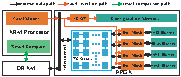
\includegraphics[width=0.99\linewidth]{system-overview}}
    \caption{Overview of the fault analysis system}
\vspace{-0.5em}
\label{fig:fault-analysis-overview}
\end{figure}

On top of the baseline FPGA-based neural network acceleration system, 
we also need a fault injection module as shown in 
Figure \ref{fig:fault-analyis-overview}. The fault injection data path 
is marked with orange arrows. It is implemented on both the ARM processor 
and FPGA. On the ARM processor part, it defines both the fault models 
such as bit-flip, stuck-at-0, and stuck-at-1, and the fault distribution 
models which determine the locations of the faults to be injected. Then it
generates the errors to be injected. On the FPGA part, the generated errors 
are sent to the FPGA from an AXI port accordingly. While errors in FPGAs are mainly 
located on the four different memory types including configuration memory, 
block memory, distributed memory and Flip-Flops. Currently, we randomly 
inject persistent errors to the first three memory types. Flip-Flops that 
get updated frequently are not handled in this work. 

For FPGA configuration memory, we take advantage of Xilinx ICAP 
port \cite{UG953}, which allows user logic to access configuration 
memory, to inject errors. While Xilinx FPGA bitstream is organized 
as frames and each frame includes configuration bits of a block of 
FPGA, we randomly choose the frame and the number of bits for each 
bit error injection. The error can be located at any place of the 
FPGA configuration memory including the regions that are not utilized.
When the position of an error is determined, we read the whole frame 
out of the configuration memory via AXI port of AXI-HWICAP \cite{PG134}, 
change the victim bit in the frame, and write it back to the configuration 
memory \cite{UG470}. This is done before the fault analysis, but it is also 
possible to do it at run-time.

For the block RAM and distributed memory, we develop an error injection 
mask (Err. Mask) which can be added to an on-chip memory block without 
changing the memory interface nor the pipelining. Meanwhile, it has an 
AXI slace port allowing ARM processor to flip a bit of any data in the 
memory block during reading. Figure \ref{fig:error-mask} shows the design 
of the error mask. Basically, it has a set of address and mask registers 
that can be configured using the attached AXI port. The addresses in 
the registers represent the position of errors to be injected while 
the corresponding masks keep the exact error bits. Whenever there is 
a read request coming to the block RAM, the read address will be compared 
with all the addresses in the registers. when there is an address match, 
the data read from the block RAM will be XORed with the mask.
Then the result will be used as the output of the block RAM 
affected by injected errors. The registers in the error mask 
can be configured in advance or at run-time. 

\begin{figure}
    \center{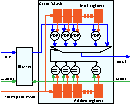
\includegraphics[width=0.7\linewidth]{error-mask}}
    \caption{Error mask for fault injection to on-chip memory}
\vspace{-0.5em}
\label{fig:error-mask}
\end{figure}

Another important part of the fault analysis platform is the result 
collection and comparison. We have the output of neural networks 
stored in the shared DRAM, which can be easily accessed on the ARM processor 
and compared to the pre-calculated golden reference. In addition, the computing 
results produced in the intermediate layers can also be compared.
The result comparison is mainly performed on the ARM processor and can be 
easily utilized for further analysis by high-level application designers.

\subsection{System fault classification}
Prior fault analysis works usually focus on computing errors of the neural networks 
and the incurred prediction accuracy loss. We argue that the consequences 
of hardware faults on a DNN acceleration system vary and should be classified 
into more categories. Table \ref{tab:classification} shows the proposed classification.
From the perspective of a system, the consequences caused by hardware faults 
roughly include system exception and accuracy degradation. System exception 
indicates that the neural network execution behaves abnormally, 
which may be stalled without returning or returns too fast or too slow.
Basically, we define them as system stall and abnormal runtime.
For the accuracy degradation, we
further classified into two cases including system stall 
and abnormal runtime.i

\begin{table}
    \centering
    \caption{Caption}
    \label{tab:classification}
    \begin{tabular}{c|cccc}
    \hline
      \multirow{2}{*}{system exception} & system stall\\
      \cline{2-2}
      & abnormal runtime\\
      \cline{1-2}
      \multirow{3}{*}{Accuracy degradation} &$$L0$\\
      \cline{2-2}
      & ... \\
      \cline{2-2}
      &$L_{k}$\\
      \cline{1-2}
      \hline
    \end{tabular}
\end{table}

We chose Neural Networks in four different application 
scenarios and try to analyze the differences of error 
tolerance in different application scenarios and networks. 
The four network applications include ResNet network for 
image classification, YOLO system for target detection, 
LSTM network for voice classification, and DCGAN network 
for image generation. We will evaluate their fault 
tolerance from accuracy and output consistency.

Neural Network accelerators injected with hardware errors 
may produce unexpected conditions. We define the system 
halt situation, which refers to a serious error in the 
system, or working improperly. such as unable to read and 
write registers, timeout, abnormal short runtime, etc. When 
the system halts, we need to reset the FPGA and restart the 
system. System halt situations are considered the result of 
errors in the evaluation of network accuracy and are listed 
separately in the output consistency.

Network accuracy refers to the overall accuracy of the 
network when performing corresponding tasks, such as the 
accuracy of 20,000 image recognition. When there are errors 
in the operation, the accuracy of the network will show a 
downward trend. For classification networks including 
ResNet and LSTM, top-5 accuracy is used to evaluate their 
accuracy, and for the YOLO system, mAP is adopted.

Output consistency is the difference between the result of 
running with errors injected and the result of normal 
running. We ran the corresponding data set when no errors 
are injected into each network at first, and defined the 
results as standard output. The results of Neural Networks 
prediction injected with errors are divided into two 
categories: result with deviation and result match. Result 
with deviation refers to system works properly with output 
differently from standard output. Result match means that 
the system works properly and the outputs are still 
standard output.

For the result with deviation case, we define its deviation 
quantitatively and further subdivide the result. Due to the 
different application functions of each network, the 
evaluation criteria of deviation are also different. For 
YOLO system, the result is the target detection bounding 
box, and when the detection result does not match the 
standard output in object type, it is defined as detection 
result error. When the result target type is consistent, 
the error is defined as the intersection area of the error 
output and the standard output divided by the area of the 
union. Target types not match for one single level, the two 
do not overlap with each other for one level, and then each 
20\% is divided into one level. For ResNet and LSTM, the 
outputs are top-5 labels. When the error output is not 
completely consistent with the standard output, the number 
of elements in the intersection of the two is taken, and 
divide the levels refer to the number. For DCGAN, we used 
the universal SSIM standard, and divided it into six levels 
according to the actual visual effects: 0~10\%, almost 
impossible to recognize; 10~20\%, barely visible; 20~50\%, 
with large deformation or distortion; 50~80\% with partial 
deformation or distortion; 80~90\%, small deformation or 
distortion can be seen; 90~100\%, almost no deformation or 
distortion is visible.
